\documentclass[
a4paper,     %% defines the paper size: a4paper (default), a5paper, letterpaper, ...
% landscape,   %% sets the orientation to landscape
% twoside,     %% changes to a two-page-layout (alternatively: oneside)
% twocolumn,   %% changes to a two-column-layout
% headsepline, %% add a horizontal line below the column title
% footsepline, %% add a horizontal line above the page footer
 titlepage,   %% only the titlepage (using titlepage-environment) appears on the first page (alternatively: notitlepage)
% parskip,     %% insert an empty line between two paragraphs (alternatively: halfparskip, ...)
% leqno,       %% equation numbers left (instead of right)
% fleqn,       %% equation left-justified (instead of centered)
% tablecaptionabove, %% captions of tables are above the tables (alternatively: tablecaptionbelow)
% draft,       %% produce only a draft version (mark lines that need manual edition and don't show graphics)
% 10pt         %% set default font size to 10 point
% 11pt         %% set default font size to 11 point
12pt           %% set default font size to 12 point
]{scrartcl}  %% article, see KOMA documentation (scrguide.dvi)

\usepackage{amsmath,stmaryrd,amsthm,amssymb} % Math packages
\usepackage{mathtools}
\usepackage{enumitem}

\newcommand{\norm}[1]{\left\Vert#1\right\Vert}
\newcommand{\abs}[1]{\lvert #1 \rvert}
\newcommand{\diag}[1]{\mathrm{diag}(#1)}
\newcommand{\defeq}{\vcentcolon=}
\newcommand{\eqdef}{=\vcentcolon}
\newcommand{\q}[1]{\dq#1\dq}            
           

  


%%% graphicx: support for graphics
\usepackage[pdftex]{graphicx}
\usepackage{caption}
\usepackage{subcaption}




%%% hyperref (hyperlinks in PDF)
\usepackage[
    hidelinks,
    backref,                     %% adds a backlink text to the end of each item in the bibliography
    pagebackref=false,           %% if true, creates backward references as a list of page numbers in the bibliography
    colorlinks=false,            %% turn on colored links (true is better for on-screen reading, false is better for printout versions)
    bookmarks=true,              %% if true, generate PDF bookmarks (requires two passes of pdflatex)
    bookmarksopen=false,         %% if true, show all PDF bookmarks expanded
    bookmarksnumbered=false,     %% if true, add the section numbers to the bookmarks
    pdfpagemode                  %% None, UseOutlines (=show bookmarks), UseThumbs (show thumbnails), FullScreen
    ]{hyperref}




%%% sets the PDF-Information options
%%% (see fields in Acrobat Reader: ``File -> Document properties -> Summary'')
%%% Note: this method is better than as options of the hyperref-package (options are expanded correctly)
\hypersetup{
  pdftitle={A Neural Network for RPCA}
  pdfauthor={Eric Brunner, Aron Distelzweig, Mirko Grimm, Bastian Schnitzer, Simon Beyer}
}



%% Use biber instead of BibTeX, see README
\usepackage[citestyle=numeric-comp,style=numeric-comp,backend=biber,sorting=none]{biblatex}
\addbibresource{handout.bib}


%----------------------------------------------------------------------------------------
%	DOCUMENT MARGINS
%----------------------------------------------------------------------------------------

\usepackage{geometry} % Required for adjusting page dimensions and margins

\geometry{
	paper=a4paper, % Paper size, change to letterpaper for US letter size
	top=2.5cm, % Top margin
	bottom=3cm, % Bottom margin
	left=2.5cm, % Left margin
	right=2.5cm, % Right margin
	headheight=14pt, % Header height
	footskip=1.5cm, % Space from the bottom margin to the baseline of the footer
	headsep=1.2cm, % Space from the top margin to the baseline of the header
}

%----------------------------------------------------------------------------------------
%	FONTS
%----------------------------------------------------------------------------------------

\usepackage[utf8]{inputenc} % Required for inputting international characters
\usepackage[T1]{fontenc} % Output font encoding for international characters
\usepackage[english,german]{babel}
\usepackage{csquotes}
\usepackage[ cal = cm,
             scr = euler
           ]{mathalfa}
           
\numberwithin{equation}{section}


\renewcommand\thefootnote{\textcolor{blue}{\arabic{footnote}}}


\setlength{\parindent}{0pt}
\setlength{\parskip}{1em}


\begin{document}
 \selectlanguage{english}
\pagenumbering{roman} %% small roman page numbers
\setcounter{page}{0}
%%% include the title
\begin{titlepage}
	\centering
	{\scshape\Huge Albert-Ludwigs-Universität Freiburg \par}
	\vspace{1,5cm}
	{\huge\bfseries A Neural Network for RPCA\par}
	\vspace{1cm}
	{\scshape\LARGE A project in \par}
	{\scshape\LARGE Stochastic Machine Learning \par}
	\vspace{10cm}
	{\Large\itshape Eric Brunner, Aron Distelzweig, Mirko Grimm, Bastian Schnitzer, Simon Beyer\par}
    \vspace{2cm}
	{\large \today\par}
\end{titlepage}

\newpage
\tableofcontents

%%% start a new page and display the list of figures
% \newpage
% \listoffigures

%%% start a new page and display the list of tables
% \newpage
% \listoftables

%%% display the main document on a new page 
\newpage
\pagenumbering{arabic} %% normal page numbers (include it, if roman was used above)

\section{Introduction}

In Principal Component Analysis (PCA) we aim at finding the principal components of a set of data points. The principal components of a set of points in $\mathbb{R}^n$ are a sequence of $n$ vectors. They are recursively defined as the $i^{th}$ vector being the direction of a line that best fits the data while being orthogonal to the first $i-1$ vectors. The line is obtained through minimizing its average squared distance from the data points. Intuitively, one can think of PCA as fitting a p-dimensional ellipsoid to the data, where each axis of the ellipsoid represents a principal component. Mathematically this corresponds to the eigenvectors of the datas' covariance matrix. Hence, the principal components form an orthonormal basis of the space $\mathbb{R}^n$. PCA is heavily used as an exploratory tool in data analysis. One big application is in quantitative finance (or generally time series analysis), where one is interested in the principal components of the empirical covariance matrix of certain financial assets. Focusing only on the largest principal components, which still hold the most important information about the data, leads to a dimensional reduction of the large dataset such that an efficient analysis of the data is still feasible.

In this project we specifically look at a modification of PCA, which is the Robust Principal Component Analysis. Here our aim is to recover a low rank Matrix $L$ from, possibly highly, corrupted matrices $M$, in the sense that some matrix entries are faulty, for example through imprecise measurements. More precisely, we start with a data matrix (or its covariance matrix) $M \in \mathbb{R}^{m \times n}$ with corrupted entries and attempt to find a decomposition into a sum $M = L + S$. $L$ is a matrix of low rank while the corrupted entries are filtered out into a sparse matrix $S$ (which means that a lot of entries are zero). In this project we will restrict to the RPCA of symmetric positive semi-definite matrices $M$, which are for example given as empirical covariance matrices.

The usual state-of-the-art algorithms for (R)PCA are computationally demanding and, hence, impractical in some applications like finance, where instantaneous calculation might be required. Therefore, the use of a neuronal network is seen to yield a valuable alternative for the design an efficient decomposition tool. In this project our aim is to implement the algorithm "Denise" (see \cite{herrera2020denise}) that aims at solving the robust PCA for semi-definite matrices through direct learning of the decomposition map $M\mapsto L+S$ via a deep neural network. We train Denise on a randomly generated synthetic dataset and evaluate the performance of the deep neural network on synthetic and real-world covariance matrices. The advantage of a neural network compared to the standard methods is that once trained the neural network delivers a function that outputs the desired decomposition of a dataset instantaneously, where using standard methods like convex optimization are computationally expensive. The algorithms are matrix specific (meaning that one has to use the algorithm for every new data), which is, therefore, very slow especially when data becomes large. For example in finance, one needs robust low rank estimation of covariance matrices of hundreds of assets instantaneously where the high performance of a neural network is very practical. As argued in \cite{herrera2020denise}, the results achieved by Denise are comparable to several state-of-the-art algorithms in terms of decomposition quality but outperforms all existing algorithms by computation time. As explained above, this is achieved by learning a single evaluation function that takes a matrix as an input and outputs the desired decomposition.

In section \ref{sec:algorithm} the considered algorithm is explained in detail. Especially we introduce the objective function on which we train the neural network and describe the network architecture. Subsequently in section \ref{sec:comparison} we introduce the principal component pursuit (PCP) algorithm, which will be used as benchmark to asses the performance of the neural networks approach. We evaluate PCP as well as the trained Denise network on a Portfolio correlation matrix of five exemplary stocks in the DAX 30 and compare the resulting decompositions. Finally, in section \ref{sec:outlook}, we summarize approaches on how to develop our project further, and which additional tasks we would like to carry out in the course of this semester.






\section{Denise}\label{sec:algorithm}

We consider $\mathbb{S}_n \subseteq \mathbb{R}^{n \times n}$ to be the set of $n$-by-$n$ symmetric matrices and $P_n\subseteq \mathbb{S}_n$ to be the subset of positive semi-definite matrices and $P_{k,n} \subseteq P_n$ the subset of matrices with rank at most $k$. As the input of our deep neuronal network we consider a Matrix $M = [M_{i,j}]_{i,j} \in P_n$. $M$ is to be decomposed as a sum $M = L + S$ where $L = [L_{i,j}]_{i,j} \in P_{k,n}$ is of rank at most $k$ and a sparse matrix $S = [S_{i,j}]_{i,j} \in P_n$. Since $L$ is assumed to be symmetric, by the Cholesky decomposition, we can represent it as $L=UU^T$, where $U = [U_{i,j}]_{i,j} \in \mathbb{R}^{n \times k}$. Therefore $M$ can be expressed as $M = UU^T + S$.

\paragraph{Loss function}
We input $M$ in the neural network, which should faithfully output the low rank matrix $U$. Hence, we want to minimize the difference between $M$ and $UU^T$, which is equal to $S$. A convenient choice of loss-function for the considered neural network is, therefore, given by the $l_1$-matrix-norm of $S$
\[
\Vert UU^T - M \Vert_{l_1} = \Vert S \Vert_{l_1}
\]
The $l_1$-norm is a common choice to guarantee sparsity of $S$.

\paragraph{Architecture}
As the matrix M is symmetric, we can reduce the input from $n^2$ to $n(n + 1)/2$ by taking the triangular lower matrix of $M$. The lower matrix is then transformed into a vector using the operator h:
\[
h: S^n \to \mathbb{R}^{n(n+1)/2}, \, M \mapsto (M_{1,1},M_{2,1},M_{2,2},\dots,M_{n,1},\dots,M_{n,n})^T
\]
Similarly we convert the output vector of the neural network into a matrix with the operator g defined as
\[
g : \mathbb{R}^{nk} \to \mathbb{R}^{n \times k}, \, X \mapsto \begin{pmatrix} X_1 & \cdots & X_k \\ \vdots & & \vdots \\ X_{(n-1)k + 1} & \cdots& X_{(n-1)k+k}\end{pmatrix}
\]
Besides the output layer, our multi-layer feed-forward neural network $\mathcal{N}: \mathbb{R}^{n(n+1)/2} \to \mathbb{R}^{nk} $ has three hidden dense layers, each exhibiting ReLU-activation function and $n/2$ nodes. Using $h$ and $g$ the matrix $U$ is the output of the neural network $U = g(\mathcal{N}(h(M)))$ and we  get the desired matrix $L=\rho(\mathcal{N}(h(M)))$ for
\[
\rho : \mathbb{R}^{rd} \to P_{r,d}, X \mapsto g(X)g(X)^T
\]


\paragraph{Generation of training data}


\newpage
\section{Testing and Comparison}\label{sec:comparison}
After the neural network has been trained with the synthetic data, as described in section \ref{sec:algorithm}, it can be tested on synthetic data, where the decomposition is known by construction, as well as on real world data. To compare the decompositions of real world data, another algorithm is needed for benchmarking, which calculates the decomposition of an arbitrary positive semidefinite matrix $M$ into a low rank, symmetric and positive-semidefinite matrix $L_0$ plus a sparse matrix $S_0$:
\begin{align}
 M = L_0 + S_0.
\end{align}
With \textit{Principal  Component  Pursuit} (PCP), there exists an algorithm, which, under some suitable assumptions, calculates the decomposition exactly via singular value decomposition (SVD) \cite{candes2009robust}. The assumptions and the main ideas of this algorithm is presented in the first subsection. In the second subsection the results of the decomposition of portfolio correlation matrices via the AI algorithm Denise with the results of the Principal Component  Pursuit algorithm.

\subsection{The Minimization Problem solved by PCP}\label{sec:pcpproblem}
Let $M$ be a given element of $\mathbb R^{n_1\times n_2}$. $\norm \cdot_*$ denotes the nuclear norm, i.e. the sum over the singular values of a matrix $\norm M_* \defeq \sum_i \sigma_i(M)$. $\norm \cdot_1$ is the well known $\ell_1$ norm $\norm M_1 = \sum_{ij} \abs{M_{ij}}$. The PCP algorithm solves the convex optimazation problem
\begin{align}
\label{pcpoptproblem}
 \mathrm{minimize} \quad \norm L_* + \norm S_1, \quad \text{where } L+S=M
\end{align}
exactly, if the the low-rank component $L_0$ fulfills a \q{incoherence} condition, and that the sparse component is \q{reasonably sparse}. The meaning of this \q{incoherence} condition for $L_0$ and the \q{reasonable} sparsity of $S_0$ is explained in \cite[subsection 1.3]{candes2009robust}. We summarize the main points real for quadratic matrices:
\par
\begin{enumerate}[label=(\roman*),ref=(\roman*)]
 \item \label{incoherencecond} Let $U\Sigma V^\top$ the singular singular value decomposition of $L_0 \in R^{n\times n}$ with rank $k\ge n$, i.e.
\begin{align}
 L_0 = U\Sigma V^\top = \sum_{i=1}^k \sigma_i u_i v_i^\top,
\end{align}
where $U=(u_1,\dots,u_k),V=(v_1,\dots,v_k) \in \mathrm{O}(n)$, $\Sigma=\diag{\sigma_1,\dots,\sigma_r,0,\dots,0} \in \mathbb R^{n\times n}$. $\sigma_1,\dots,\sigma_k$ are the singular values and $u_i$ and $v_i$, $i=1,\dots,k$, are the left-singular and right-singular vectors for $\sigma_i$, respectively. Then the matrix $L_0$ is called incoherent, with parameter $\mu$, if
\begin{align}
 \max_i \norm{U e_i}^2 \ge \dfrac{\mu k}{n^2},\quad  \max_i \norm{V e_i}^2 \ge \dfrac{\mu k}{n^2}, \quad \norm{UV^\top}_\infty \ge \dfrac{\sqrt{\mu k}}{n}.
\end{align}
$e_i$ are the canonical basis vectors of $\mathbb R^n$. 
 \item \label{uniformlysparse} The positions of the nonzero elements of the sparsity matrix are selected uniformly random.
\end{enumerate}
If \ref{incoherencecond} is fulfilled, the matrix $L_0$ is considered as not sparse. With \ref{uniformlysparse} we try to prevent, that the nonzero elements are only in one, or few columns of the sparsity matrix. For example if the entries of $S_0$ except the first column are all zero, and the first column of $S_0$ is the negative of the first column of $L_0$, then it is impossible to recover the low rank component and sparse component exactly. To avoid, such variety of possibilities for the decomposition 
\ref{uniformlysparse} is a reasonable assumption.

\subsection{PCP Algorithm}\label{sec:pcpalgorithm}
\label{sec:PCP}
In this subsection, a brief description of the PCP algorithm, which we use for comparison with Denise, is given. There are different strategies to solve the problem \eqref{pcpoptproblem} numerically. As described in \cite{candes2009robust}, we consider an \textit{augmented Lagrange multiplier}. This is why Candes et al. named this method the ALM method. \eqref{pcpoptproblem} is equivalent to the minimization of the following \textit{augmented Lagrangian}
\begin{align}
 \mathcal L(L,S,Y) = \norm L_* + \lambda \norm S_1 + \langle Y, M -L - S \rangle + \dfrac{\mu}{2} \norm{M - L - S}_F^2.
\end{align}
Here $\langle \cdot, \cdot \rangle$ is defined as 
%$\langle A , B \rangle = \trace{A^\top B}$
$\langle A , B \rangle = \trace{A^\top B}$
, with real quadratic matrices $A,B$. $\norm \cdot_F$ is the Frobenius norm. One can show, that
\begin{alignat}{2}
 &\arg \min_S \mathcal L(L,S,Y) &&= \mathcal S_{\lambda \mu}(M-L+ \mu^{-1} Y), \\
 &\arg \min_L \mathcal L(L,S,Y) &&= \mathcal D_\mu (M-S-\mu^{-1} Y),
\end{alignat}
where $\mathcal S_\tau : \mathbb R^{n \times n} \to \mathbb R^{n \times n}: (X_{ij})_{ij} \mapsto (\sgn{X_{ij}} \max \left( \abs{X_{ij}} - \tau,0 \right))_{ij}$, is the extension of the shrinkage operator in $\mathbb R$ to $\mathbb R^{n \times n}$. $\mathcal D_\tau (X)$ is defined as $\mathcal D_\tau (X) = U \mathcal S_\tau (\Sigma) V^\top$, where $U \Sigma V^\top$ is the SVD of $X$. Hence, the following algorithm, taken from \cite[29]{candes2009robust}, is productive
\begin{enumerate}
 \item \textbf{Initialize}: $\mathrm S_0 = Y_0 = 0,\mu >0$.
 \item \textbf{While} not converged \textbf{do}
    \begin{subequations}
    \begin{alignat}{2}
     &L_{k+1} &&= \mathcal D_\mu(M-S_k-\mu^{-1} Y_k) \\
     &S_{k+1} &&= \mathcal S_{\lambda \mu}(M-L_{k+1} +\mu^{-1} Y_k) \\
     &Y_{k+1} &&= Y_k + \mu(M-L_{k+1} - S_{k+1})
    \end{alignat}
    \end{subequations}
 \item \textbf{Return}: L,S.
\end{enumerate}
With the calculations of the second step, it is avoided to solve a sequence of convex programs. To archieve good relativ accuracy, only a few iteration steps are neccessary \cite[section 3]{candes2009robust}.

\subsection{Portfolio Correlations from DAX 30 with PCP and Denise}

\textcolor{red}{Sparsity-values}

\textcolor{red}{Are the matrices the same as in the plot? Corr = Cov ?}

For test purposes we applied the PCP algorithm to the empirical covariance matrix based on the prices of five share certificates of the companies Allianz, BASF Bayer, Beiersdorf and BMW  of the last six months. The following covariance matrix is obtained
\begin{align}
 &(\mathrm{Corr}(x_i,x_j))_{i,j} \notag \\
 &= \begin{pmatrix} 142.67041515&  28.06338926&  30.56147946&   2.52487121&
         31.18558268\\  28.06338926&  14.54671933& -10.75409144&  -2.97700557&
         20.0735403 \\  30.56147946& -10.75409144&  65.84451884&  11.30075662&
        -28.04105723\\   2.52487121&  -2.97700557&  11.30075662&  10.38498412&
         -5.84017695\\  31.18558268&  20.0735403 & -28.04105723&  -5.84017695&
         33.39091805 \end{pmatrix},
\end{align}
where $x = (x_1,\dots,x_5) =(\text{Allianz, BASF Bayer, Beiersdorf, BMW})$. The PCP algorithm returns the decomposition
\begin{align}
 L_0 &= \begin{pmatrix}
       33.15288862&  19.03429426&  -2.38353047&   2.5249416 &
         24.04138395\\
         19.03429426&  14.54671744& -10.7540876 &  -2.97707117&
         20.07354269\\
         -2.38353047& -10.7540876 &  24.51612531&  11.30069593&
        -17.99311351\\ 
        2.5249416 &  -2.97707117&  11.30069593&   5.60790277&
         -5.84023382\\
         24.04138395&  20.07354269& -17.99311351&  -5.84023382&
         28.30038404
       \end{pmatrix},
       \\
S_0 &=\begin{pmatrix}109.51752654&   9.029095  &  32.94500994&   0.        &
          7.14419873\\ 9.029095  &   0.        &  -0.        &  -0.        &
         -0.\\ 32.94500994&  -0.        &  41.32839353&   0.        &
        -10.04794373 \\ 0.        &  -0.        &   0.        &   4.77708135&
          0.        \\ 7.14419873&  -0.        & -10.04794373&   0.        &
          5.09053401
       \end{pmatrix}.
\end{align}
The rank of $L_0$ is $2$. This is obviously a exact decomposition $(\mathrm{Cov}(x_i,x_j))_{i,j} = L_0 + S_0$.

The comparison of the RPCA decomposition of the covariance matrix $M = Cov$ into rank $2$ matrix $L$ and sparse $S$ is show in Fig. \ref{fig:comp_finance}. As one can see, the decomposition obtained from our neural network suffers from one significant outlier (the bottom right matrix element) in $L$ as well as $S$, which is not apparent in the PCP decomposition. Due to this outlier not much structure is visible in $L$ obtained from the neural network. However, apart from the bottom right matrix elements the $S$-matrices of both methods seem to agree to some approximation (respecting the corresponding color code). This will be analyzed in more detail in future work.

\begin{figure}
	\centering
	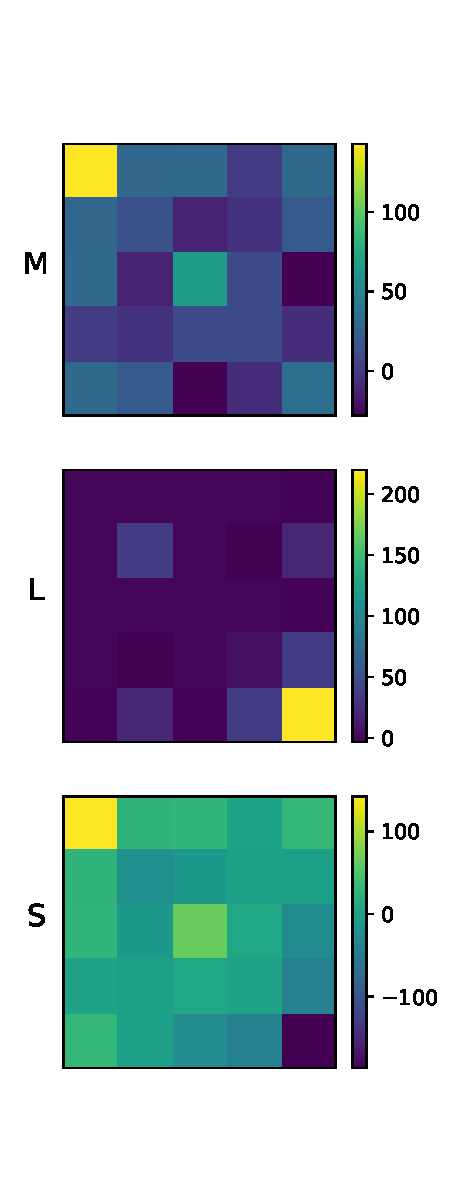
\includegraphics[width=0.48\textwidth]{fig/denise_output_finance.pdf}
	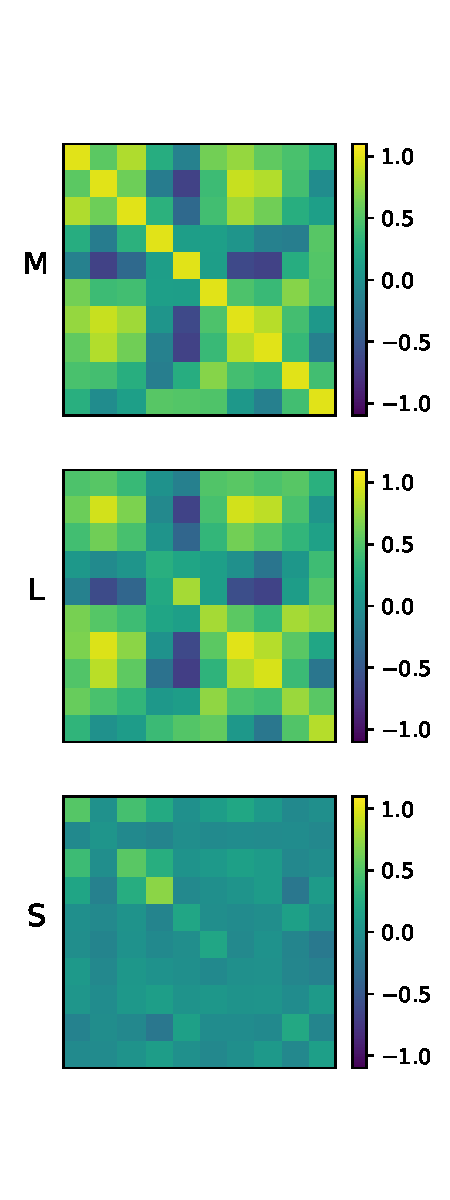
\includegraphics[width=0.48\textwidth]{fig/pcp_output_finance.pdf}
	\caption{Comparison of RPCA of the empirical $5\times 5$ covariance matrix of the prices of five share certificates (see main text) from the DAX 30. The left panel shows the resulting decomposition $M=L+S$ obtained from the neural network approach, while the right panel shows the results from PCP.}
	\label{fig:comp_finance}
\end{figure}


\subsection{Covariance matrix of personality features with PCP and Denise}
Here we compare the performance of the RPCA of our neural network approach and the benchmark PCP algorithm on personality feature obtained from \textcolor{red}{??} individuals.

\textcolor{red}{which personality features}

From the data we determine their empirical covariance matrix $M$. As in the previous subsection, we calculate the RPCA-decomposition $M=L + S$ by means of our neural network approach as well as by using the PCP method introduced in \ref{sec:pcpalgorithm}. The obtained low rank matrix $L$ and the sparse part $S$ containing corruptions of the input matrix are shown in Fig. \ref{fig:comp_psych}.

\textcolor{red}{which rank}

As in the analysis of the financial data, the neural network decomposition exhibits very few strong outliers, which suppress the visual structure of the obtained matrices $L,S$ to some extend. As before, these outliers are not present in the PCP results. Hence, the PCP-method seems to function more stable than the network ansatz. \textcolor{red}{oreover, the sparsity of $S$ obtained from PCP is lower than from the neural network decomposition, indicating a performance advantage of PCP.}

The comparison of both methods, in combination with the striking results reported in \cite{herrera2020denise}, may be explained by a sub-optimal choice of network-architecture (to few nodes per hidden layer) of our network. Another source of instability might result from the small training sets or not ideally chosen hyper-parameters such as batch-size. This will be analyzed in detail in future work.





\begin{figure}
	\centering
	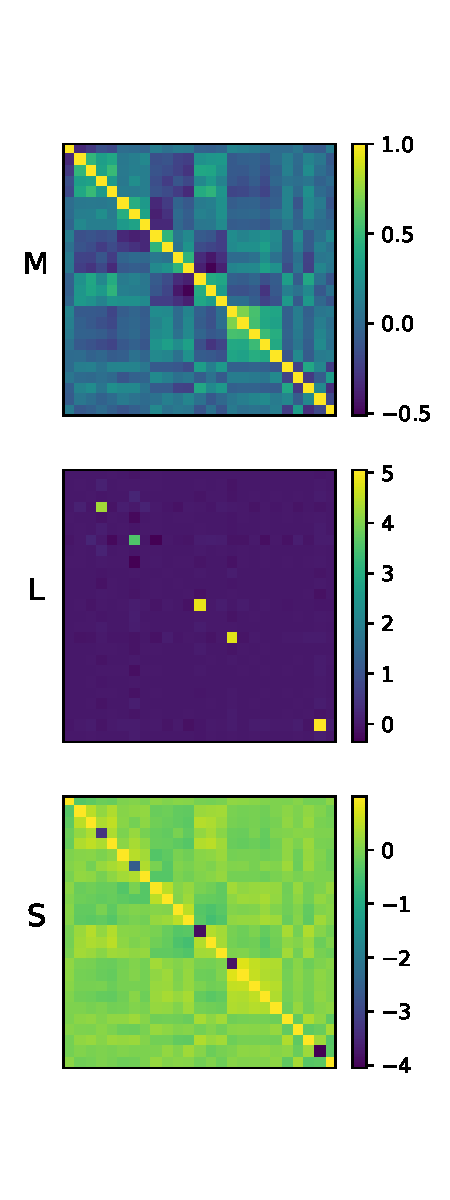
\includegraphics[width=0.48\textwidth]{fig/denise_output_psych.pdf}
	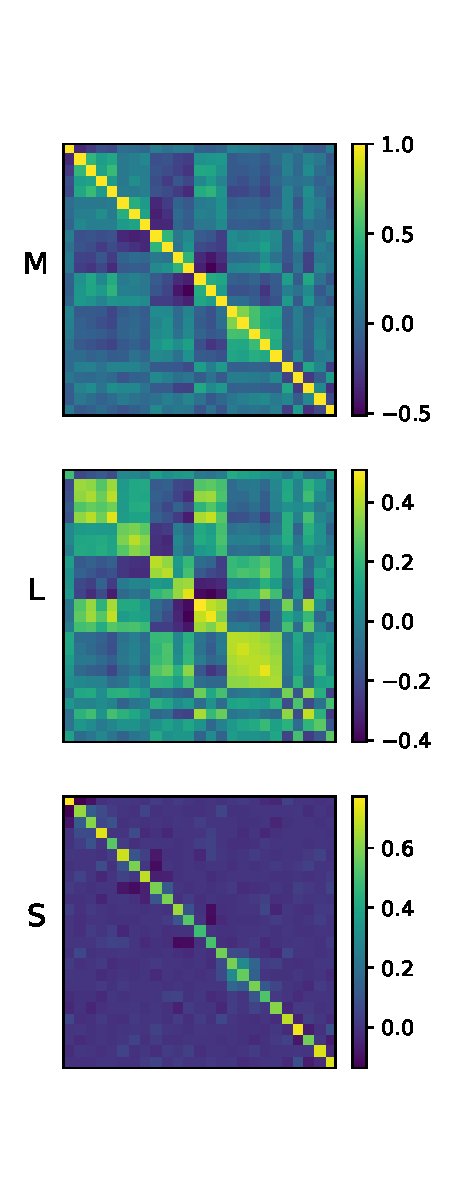
\includegraphics[width=0.48\textwidth]{fig/pcp_output_psych.pdf}
	\caption{Comparison of RPCA of the empirical $27\times 27$ covariance matrix of 27 personality features of \textcolor{red}{???} individuals (see main text). The left panel shows the resulting decomposition $M=L+S$ obtained from the neural network approach, while the right panel shows the results from PCP.}
	\label{fig:comp_psych}
\end{figure}









\section{Outlook}


\newpage


% \bibliographystyle{unsrt}
\printbibliography[heading=bibintoc]
 
 
\end{document}
